\chapter{Redes Neuronales y Modelos Generativos}\label{chap:redes-neuronales-y-modelos-generativos}
{
Este capítulo introduce los conceptos esenciales acerca de los modelos generativos. Para ello, se empieza por definir qué es una red neuronal.
\section{Redes Neuronales}\label{sec:redes-Neuronales}
{
    En el último tiempo se ha visto un auge en el uso de las redes neuronales en diversas áreas de la ciencia y la tecnología. Esto se debe a que las redes neuronales han demostrado ser muy efectivas en la resolución de problemas complejos, como la clasificación de imágenes, el procesamiento de lenguaje natural, y la generación de texto e imágenes, entre otros.

    Este capítulo introduce los conceptos básicos de las redes neuronales, aunque no se profundiza\FM{Me suena raro profundiza. Está bien utilizado?} en los detalles de su funcionamiento. Para ello, se recomienda al lector revisar la literatura especializada en el tema, tales como \cite{goodfellow2016deep,calin2020deep}\FM{En este caso están bien referenciados?}.\FM{Esta sección lo hice de mis propios conocimientos y no tomé referencia de ninguna fuente. ¿Cómo podría decir esto?}

    El proceso de definición de una red neuronal comienza estableciendo algunas constantes preliminares. El origen de los nombres de las siguientes definiciones se entenderán con el Ejemplo~\ref{ex:ejemplo-red-neuronal}. Se define por $L\in\N$ la \emph{profundidad} de la red, el cuál determina el número de \textit{capas ocultas} y la \textit{capa de salida} que tiene la red. Para $\ell \in \left\{ 0,\ldots, L \right\}$, se define $d_\ell\in\N$ como el \emph{número de neuronas de la capa $\ell$}.

    De esta manera, una red neuronal prealimentada (FFNN por sus siglas en inglés: \textit{feed-forward neural net}) es simplemente una composición de funciones lineales y no lineales. Más precisamente, para $L$ funciones lineales $\{ g^{(\ell)}_{\vth_\ell} \colon \R^{d_{\ell-1}} \to \R^{d_{\ell}} \mid \ell = 1, \ldots, L \}$, definidas por
    \begin{align*}
        g^{(\ell)}_{\vth_\ell} \colon \R^{d_{\ell-1}} & \to \R^{d_\ell}                                                        \\
        \vx_\ell                                      & \mapsto g^{(\ell)}_{\vth_\ell}(\vx_\ell) = \vW_\ell \vx_\ell + b_\ell,
    \end{align*}
    donde $\vth_\ell = (\vW_\ell, b_\ell)$ corresponden a los \textit{parámetros}, $\vW_\ell \in \R^{d_{\ell} \times d_{\ell-1}}$ a los \emph{pesos} y $b_\ell \in \R^{d_\ell}$ al \emph{sesgo}\footnote{En español también se suele referir al sesgo por su anglicismo: \textit{bias}.} de la capa $\ell$.
    Se considera además $L$ funciones no lineales $\{ \sigma^{(\ell)} \colon \R \to \R \mid \ell = 1, \ldots, L \}$, a las cuales llamaremos \emph{funciones de activación}. Por convención, se asume que las funciones de activación son aplicadas elemento a elemento, es decir, que si $\sigma$ es una función de activación, entonces $\sigma(\vx) = \left( \sigma(x_1), \ldots, \sigma(x_n) \right)$ para $\vx = (x_1, \ldots, x_n) \in \R^n$.

    Estas funciones lineales y no lineales se pueden componer para formar una red neuronal:
    \begin{equation}
        f_{\vth}(\vx) = \sigma^{(L)} \circ g^{(L)}_{\vth_L} \circ \sigma^{(L-1)} \circ g^{(L-1)}_{\vth_{L-1}} \circ \cdots \circ \sigma^{(1)} \circ g^{(1)}_{\vth_{1}}(\vx).
    \end{equation}
    A este tipo de modelos se les suele representar como grafos dirigidos acíclicos, describiendo cómo las funciones se encuentran compuestas entre sí.

    \begin{remark}
        Cabe destacar que es necesario que las funciones de activación $\sigma$ sean no lineales. Pues si lo fueran, entonces la red sería una composición de funciones lineales, lo que resulta en una única función lineal. La problemática que se tendría con esta definición es que no habría ninguna ganancia con hacer la red más profunda, pues todo colapsaría a una única capa. Es por este motivo que a estas funciones se les llama \textbf{funciones de activación}, pues ``activan'' la no-linealidad de la red, permitiendo que esta pueda aprender funciones más complejas.\FM{Quizás se pueda dividir este párrafo en dos.}
    \end{remark}


    \begin{example}\label{ex:ejemplo-red-neuronal}
        En la Figura~\ref{fig:ejemplo-red-neuronal} se puede observar una representación de una red neuronal con tres capas ocultas y una capa de salida.

        \begin{figure}[htbp]
            \centering
            % \missingfigure{Ejemplo de una red neuronal}
            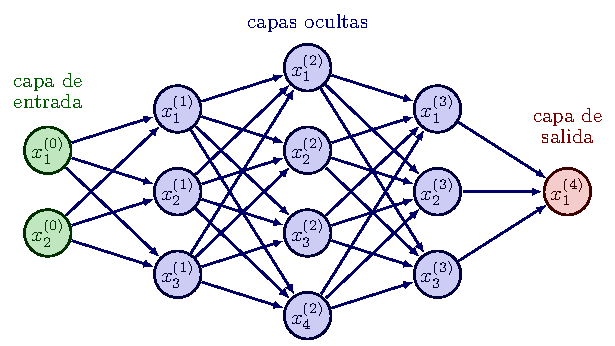
\includegraphics[width=0.5\textwidth]{img/neural_network/neural_network_feed_forward.pdf}
            \caption{Representación de una FFNN con cuatro capas. Elaboración propia.}
            \label{fig:ejemplo-red-neuronal}
        \end{figure}

        En este caso, la red neuronal se encuentra compuesta por cinco capas: una de entrada con $d_0 = 2$, tres ocultas con $d_1 = 3$, $d_2 = 4$, $d_3 = 3$, y una de salida con $d_4 = 1$. Cada uno de los nodos $x_i^{(\ell)}$ corresponde a la $i$-ésima \textit{neurona} de la capa $\ell$. Es este el motivo de porqué a $d_\ell$ se les refiere como el número de neuronas de la capa $\ell$. Además, se puede notar que, sin contar la capa de entrada, la red neural tiene una profundidad de $L = 4$ capas, de ahí que se le llame profundidad de la red.

        En este caso, la función $g^{(\ell)}_{\vth_\ell}$ es representada a través de los arcos que conectan las neuronas de la capa $\ell-1$ con las neuronas de la capa $\ell$. Por otro lado, las funciones de activación $\sigma^{(\ell)}$ se encuentran implícitamente utilizadas al definir recursivamente los vectores de neuronas $x^{(\ell)} \in \R^{d_\ell}$ de la siguiente manera:
        \begin{equation}
            x^{(\ell)} =
            \begin{cases}
                \vx,                                                         & \text{si } \ell = 0,           \\
                \sigma^{(\ell)} \circ g^{(\ell)}_{\vth_\ell} (x^{(\ell-1)}), & \text{en cualquier otro caso.}
            \end{cases}
            \quad \forall \ell = 0, \ldots, L.
        \end{equation}
        Es fácil comprobar que la salida de la red neuronal es $f_{\vth}(\vx) = x^{(L)}$.\FM{Es posible que esta línea no sea necesaria.}
    \end{example}

    La razón por la que las redes neuronales han tenido tanto éxito en los últimos años se debe a que estas son capaces de aprender funciones muy complejas, siempre y cuando se les entregue suficiente cantidad de datos y tengan la capacidad\FM{No me gusta la palabra capacidad, quisiera cambiarlo por otro nombre} de neuronas suficiente. Esto se debe a que las redes neuronales son capaces de aproximar una gran familia de funciones continuas, como lo establece George Cybenko en el 1989 en su Teorema de Aproximación Universal (UAT por sus siglas en inglés) \cite{cybenko1989approximation}.

    A pesar de que la primera versión del UAT fue propuesta por Cybenko en 1989, el teorema fue popularizado por Kurt Hornik en 1991 \cite{hornik1991approximation}. Esto debe a que en el teorema de Cybenko utiliza una función de activación sigmoide, mientras que en la versión de Hornik lo extiende a una función de activación continua. Por este motivo, es que a continuación se presenta la versión de Hornik del UAT.
    \begin{theorem}[Teorema de Aproximación Universal \cite{hornik1991approximation}]\label{thm:universal-approximation-theorem}
        Sea $\sigma \in \ContSpace[\R, \R]$ una función de activación continua.
        Sean $d_0, d_2 \in \N$, números naturales, $K \subseteq \R^{d_0}$ un conjunto compacto y $f \in \ContSpace[K, \R^{d_2}]$ la función a aproximar.
        Entonces, $\sigma$ no es polinomial sí y sólo sí para cada $\epsilon > 0$, existe $d_1\in\N$, $\vW \in \R^{d_1 \times d_0}$, $b \in \R^{d_1}$ y $C \in \R^{d_2 \times d_1}$ tal que:
        \begin{equation}
            \sup_{\vx \in K} \left\| f(\vx) - C \cdot \sigma(\vW \cdot \vx + b) \right\| < \epsilon.
        \end{equation}
    \end{theorem}

    \begin{remark}
        El Teorema~\ref{thm:universal-approximation-theorem} establece que una red neuronal de una única capa oculta con una función de activación no polinomial (como por ejemplo, una sigmoide) es capaz de aproximar cualquier función continua en un conjunto compacto $K$ con un error arbitrariamente pequeño. Sin embargo, este teorema no establece cuántas neuronas en la capa oculta son necesarias para aproximar dicha función, ni tampoco establece cómo se deben de escoger los parámetros de la red neuronal.
    \end{remark}

    A lo largo de los años, más versiones del UAT han sido propuestas, aunque el Teorema~\ref{thm:universal-approximation-theorem} ya ejemplifica\FM{No me gusta que se diga ``ejemplifica''} la idea de porqué las redes neuronales son tan efectivas en la aproximación de funciones.\FM{Este párrafo siento que es muy pequeño}

    Se terminará este capítulo mencionando que existen múltiples variantes de las redes neuronales, como las redes neuronales convolucionales (CNN por sus siglas en inglés) y las redes neuronales recurrentes (RNN por sus siglas en inglés). Estas variantes se han vuelto muy populares en el área de la visión computacional y del procesamiento de lenguaje natural, respectivamente. En lo particular, en este trabajo se hará uso \FM{En este caso, ¿debería ser ``se hará uso'' o debería ser ``se usa''?}  de las redes neuronales convolucionales.




}  % end of sec. Redes Neuronales


\section{Redes Neuronales Convolucionales}\label{sec:redes-neuronales-convolucionales}
{
    \FM[inline]{Escribir! (será necesario?)}
}  % end of sec. Redes Neuronales Convolucionales


\section{Redes Generativas Adversarias}\label{sec:redes-generativas-adversarias-GAN}
{
% Analogía ladron-policía
Comencemos esta sección imaginando la siguiente situación\footnote{Este ejemplo es una adaptación y fue inspirado de \cite[min. 4:32]{santana2017creando}}:
\begin{quotation}
    \textit{Supongamos que hay un ladrón que desea engañar a un policía entregándole un billete falso. El ladrón, que es un inexperto, le entrega una servilleta, con una cara dibujada en ella, y que en el otro lado de la servilleta tiene escrito: ``\emph{esto vale un millón de dólares}''. El policía, que ha sido entrenado en la detección de billetes falsos, revisa el billete para comprobar que, efectivamente, es un billete falso.}

    \textit{Sin embargo, en vez de enviar a la cárcel al ladrón, lo que hace es decirle al ladrón cuales fueron sus fallos, y de qué manera puede este mejorar en sus falsificaciones. Por su parte, el policía también se entrena más y más en la detección de billetes falsos, pues puede que en algún momento, el ladrón se vuelva tan bueno en la elaboración de billetes falsos, que llegue a engañar al policía con uno de sus billetes.}
\end{quotation}

\begin{figure}[htbp]
    \centering
    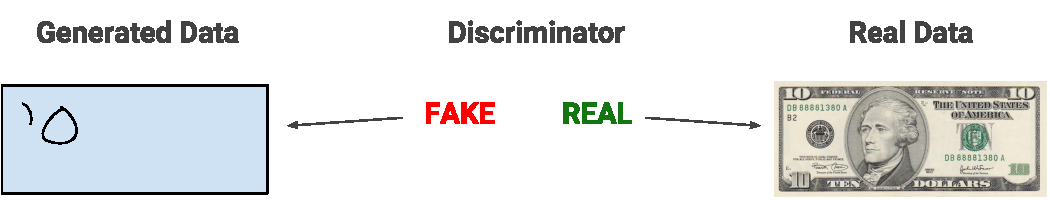
\includegraphics[width=0.7\textwidth]{img/gan/bad_gan.pdf}\vspace{0.6cm}
    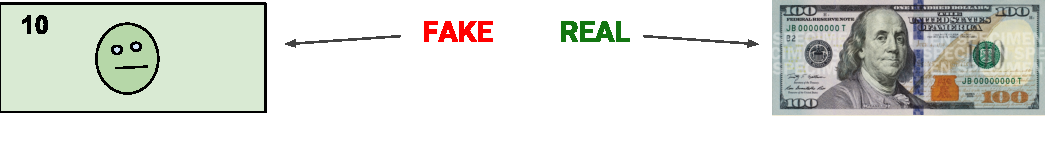
\includegraphics[width=0.7\textwidth]{img/gan/ok_gan.pdf}
    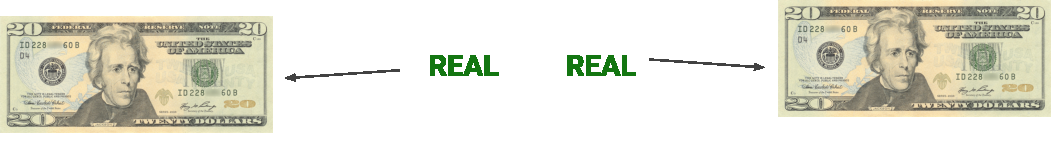
\includegraphics[width=0.7\textwidth]{img/gan/good_gan.pdf}
    \caption{Visualización gráfica de la analogía del ladrón y el policía en las GAN. Imagen obtenida de \cite{googlegan}.}
    \label{fig:gan-analogy}
\end{figure}

El marco de las Redes Generativas Adversarias (GAN), introducidos por \cite{goodfellow2014generative}, es en esencia, la analogía del ladrón y el policía.
La GAN define un juego donde el objetivo de la \emph{generadora} (el ladrón) es la de generar muestras que parezcan reales, mientras que el objetivo de la \emph{discriminadora} (el policía) es el de clasificar las muestras como verdaderas o falsas.
En este caso, la generadora se entrena para engañar a la discriminadora, y la discriminadora se entrena para detectar la falsedad de las muestras generadas.

En este trabajo de tesis se plantea una definición formal de una GAN, en el contexto no paramétrico, y utilizando medidas de probabilidades generales. Este enfoque es diferente al que se plantea en el \textit{paper} original \cite{goodfellow2014generative}, donde se utiliza una formulación no paramétrica, pero asumiendo que las medidas de probabilidad son absolutamente continuas con respecto a la medida de Lebesgue.

Por tanto, esta sección se basa en \cite{wikipediagan}\footnote{Nota del Autor: En este artículo, se menciona que las Definiciones y Teoremas planteados provienen del \textit{paper} original \cite{goodfellow2014generative}. Sin embargo, este artículo realiza una formulación diferente a tal \textit{paper}, como se mencionó anteriormente. He intentado investigar, tanto en este artículo como en la \textit{web} si es que existía algún libro o \textit{paper} del cuál se pudo haber basado el autor del artículo, pero todo parece indicar que esta formulación es original de tal autor (el cuál, además, lo realizó de forma anónima), y por tanto, considero poco ético no hacer referencia al artículo del cuál genuinamente se basa esta sección.},
el cuál senta\FM{Quiero cambiar esta palabra} las bases necesarias utilizando medidas de probabilidad generales. Sin embargo, las demostraciones y teoremas presentadas en esta sección han sido validadas y modificadas para asegurar la formalidad y correctitud de los resultados. Por este motivo, en esta sección se presentan demostraciones más detalladas que en el resto del trabajo.

Desde el punto de vista de la teoría de juegos, la GAN se define como un juego de dos jugadores: una \textit{generadora} $\Prob_G$, donde su conjunto de estrategias es $\ProbSpace[\cX]$ (con $\cX$ el \textit{conjunto de referencia}, e.g. $\cX=[0, 1]^{n_1\times n_2}$ para un conjunto de imágenes), y una \textit{discriminadora} $\Prob_D(\dd y \mid x)$, donde su conjunto de estrategias es el conjunto de kernels Markovianos.\FM{Creo que aquí podría haber un punto aparte en vez de un punto seguido.} Con esto, la GAN es un juego de suma cero con la siguiente función valor objetivo:
\begin{equation}
    \label{eq:gan-objective}
    V(\Prob_G, \Prob_D)
    = \Exp_{X\sim\Prob_G}{\Exp_{Y \sim \Prob_D(\dd y \mid X)} \left[ \ln Y \right]}
    + \Exp_{\tilde X\sim\Prob_G}{\Exp_{Y \sim \Prob_D(\dd y \mid \tilde X)} \left[ \ln (1 - Y) \right]},
\end{equation}
donde la generadora busca minimizar la función valor, mientras que la discriminadora busca maximizar esta cantidad.

El objetivo final de la generadora es el de encontrar una distribución $\Prob_G$ tal que se aproxime a una distribución de referencia $\Prob_X \in \ProbSpace[\cX]$ (del cuál se tiene acceso a través de una medida empírica $\hat \Prob_X = \frac{1}{N} \sum_{i=1}^{N} \delta_{x_i}$). Por el otro lado, el objetivo de la discriminadora es el de clasificar las muestras verdaderas y falsas, asignándole valores cercano a 1 y 0 respectivamente.

% En la práctica, la forma de implementar la generadora es a través de un \emph{modelo generativo de espacio latente}. Esto es,
% \begin{equation}
%     \Prob_G (\dd x) \eqdef \int_\cZ \Prob_G(\dd x \mid z) \; \Prob_Z \left( \dd z\right),
% \end{equation}
% donde $\cZ$ es el espacio de las variables latentes, y $\Prob_Z \in \ProbSpace[\cZ] $ es la distribución del espacio latente (típicamente se utiliza distribución Gaussiana o Uniforme). Por simplicidad, el modelo generativo $\Prob_G (\dd x \mid z)$ se mapea de forma determinista a través de $\Prob_G (\dd x \mid z) = \delta_{G(z)}(\dd x)$, a través de una función $G\colon \cZ \to \cX$.

El siguiente teorema nos habla acerca de la naturaleza del discriminador óptimo:

\begin{theorem}[El discriminador óptimo calcula la divergencia de JS]
    \label{thm:gan-optimal-discriminator}
    Para cualquier estrategia de generador $\Prob_G$ fijo, existe un único discriminador óptimo $\Prob_D^\ast$ que maximiza la función objetivo \eqref{eq:gan-objective}, el cuál toma una forma determinista por medio de $\Prob_D^\ast(\dd y \mid x) = \delta_{D^\ast(x)}(\dd y)$, donde $D^\ast(x) = \dv{\Prob_X}{(\Prob_G+\Prob_X)}$. En tal caso, la función valor toma la siguiente forma:
    \begin{equation}
        V(\Prob_G, \Prob_D^\ast) = \JS{\Prob_X}{\Prob_G} - 2 \ln 2.
    \end{equation}
\end{theorem}

Este teorema nos dice que el discriminador óptimo es aquel que calcula la divergencia de Jensen-Shannon entre la distribución de referencia $\Prob_X$ y la distribución generada $\Prob_G$, salvo una constante. Además, nos dice que el discriminador toma una forma determinista, de forma que bastaría con buscar una función (como por ejemplo, una red neuronal) $D\colon\cX\to [0, 1]$ tal que la aproxime.

La siguiente demostración se basa en \cite{wikipediagan}, el cuál se han agregado detalles para mayor comprensión y formalidad.

\begin{proof}[Demostración del Teorema~\ref{thm:gan-optimal-discriminator}]
    Dado $X \sim \Prob_X$, por la desigualdad de Jensen se tiene que:
    \begin{equation}\label{eq:gan-jensen-inequality-1}
        \Exp_{Y \sim \Prob_D \left( \dd y \mid X \right)} \left[ \ln Y \right]
        \leq \ln \left( \Exp_{Y \sim \Prob_D \left( \dd y \mid X \right)} \left[ Y \right] \right).
    \end{equation}
    Análogamente, dado $\tilde X \sim \Prob_G$, se tiene que:
    \begin{equation}\label{eq:gan-jensen-inequality-2}
        \Exp_{Y \sim \Prob_D ( \dd y \mid \tilde X )} \left[ \ln \qty\big(1 - Y) \right]
        \leq \ln \left( \Exp_{Y \sim \Prob_D ( \dd y \mid \tilde X )} \left[ 1 - Y \right] \right).
    \end{equation}
    Por el lema de Doob \cite[Ver pág. 316, Cor. 9.4.11]{san2018teoria}, se sabe que existe una función $D \colon \cX \to [0, 1]$ tal que $\Exp_{Y \sim \Prob_D \left( \dd y \mid X \right)} \left[ Y \right]
        = D(X)$,
    % \begin{equation}
    %     \Exp_{Y \sim \Prob_D \left( \dd y \mid X \right)} \left[ Y \right]
    %     = D(X),
    % \end{equation}
    es decir, que el discriminador toma una forma determinista $\Prob_D \left( \dd y \mid x \right) = \delta_{D(x)}(\dd y)$. Utilizando esta propiedad en las desigualdades \eqref{eq:gan-jensen-inequality-1} y \eqref{eq:gan-jensen-inequality-2} y sumando, se tiene que:
    \begin{equation}
        V(\Prob_G, \Prob_D) \leq \Exp_{X \sim \Prob_X} \Big[ \ln D(X) \Big] + \Exp_{\tilde X \sim \Prob_G} \Big[ \ln \qty\big(1 - D(\tilde X)) \Big],
    \end{equation}
    y dado que la parte derecha de la desigualdad es una cota superior de la función valor, s.p.g. se puede asumir que el discriminador toma una forma determinista en el óptimo. En tal caso, la función valor toma la forma del lado derecho de la desigualdad anterior.
    % \begin{equation}
    %     V(\Prob_G, \Prob_D) = \Exp_{X \sim \Prob_X} \Big[ \ln D(X) \Big] + \Exp_{\tilde X \sim \Prob_G} \Big[ \ln \qty\big(1 - D(\tilde X)) \Big].
    % \end{equation}

    Tomando $\Prob = \Prob_X + \Prob_G$, es claro que $\Prob_X \ll \Prob$ y $\Prob_G \ll \Prob$, y por tanto, existen las derivadas de Radon-Nikodym:
    \begin{align*}
        \rho_X & = \dv{\Prob_X}{\Prob}, & \rho_G & = \dv{\Prob_G}{\Prob},
    \end{align*}
    donde claramente $\rho_X + \rho_G = 1$. En tal caso, la función valor toma la siguiente forma:
    \begin{equation}
        \label{eq:gan-objective-2}
        V(\Prob_G, \Prob_D) = \int_\cX \big[ \rho_X(x) \ln D(x) + \rho_G(x) \ln \qty(1 - D(x)) \big] \; \Prob(\dd x).
    \end{equation}
    Notemos que la función $y \mapsto a \ln y + b \ln(1-y)$ alcanza su máximo en $y^\ast = \frac{a}{a+b}$, y por tanto, la función $D^\ast$ que maximiza la función valor es:
    \begin{equation}
        D^\ast = \frac{\rho_X}{\rho_X + \rho_G} = \dv{\Prob_X}{(\Prob_X + \Prob_G)} .
    \end{equation}
    Por otro lado, si evaluamos $D^\ast$ en la función valor \eqref{eq:gan-objective-2}, se tiene que:
    \begin{align*}
        V(\Prob_G, \Prob_D^\ast)
         & = \Exp_{X \sim \Prob_X} \left[ \ln \dv{\Prob_X}{\Prob}(X) \right] + \Exp_{\tilde X \sim \Prob_G} \left[ \ln \dv{\Prob_G}{\Prob}(\tilde X) \right] \\
         & = \KL{\Prob_X}{\frac{\Prob_X + \Prob_G}{2}} - \ln 2 + \KL{\Prob_G}{\frac{\Prob_X + \Prob_G}{2}} - \ln 2                                           \\
         & = \JS{\Prob_X}{\Prob_G} - 2 \ln 2,
    \end{align*}
    lo que concluye la demostración.
\end{proof}

Dado que para cada generador $\Prob_G$ existe un único discriminador óptimo $\Prob_D^\ast$, entonces tiene sentido definir la siguiente función:
\begin{equation}
    C(\Prob_G) \eqdef V(\Prob_G, \Prob_D^\ast) = \JS{\Prob_X}{\Prob_G} - 2 \ln 2.
\end{equation}
El siguiente teorema nos dice que existe un único generador óptimo $\Prob_G^\ast$ que minimiza la función $C(\Prob_G)$, y que este corresponde a la distribución de referencia $\Prob_X$:

\begin{theorem}
    El mínimo global de la función $C(\Prob_G)$ se alcanza en $\Prob_G^\ast = \Prob_X$, y el valor mínimo es $C(\Prob_X) = - \ln 4$.
\end{theorem}

\begin{proof}
    Por el Teorema anterior, se tiene que:
    \begin{align*}
        \min_{\Prob_G} \max_{\Prob_D} V(\Prob_G, \Prob_D)
         & = \min_{\Prob_G} V(\Prob_G, \Prob_D^\ast)         \\
         & = \min_{\Prob_G} C(\Prob_G)                       \\
         & = \min_{\Prob_G} \JS{\Prob_X}{\Prob_G} - 2 \ln 2.
    \end{align*}
    Como la divergencia de Jensen-Shannon es estrictamente positiva si $\Prob_G \neq \Prob_X$, y nula si $\Prob_G = \Prob_X$, entonces se tiene que el mínimo global de la función $C(\Prob_G)$ se alcanza en $\Prob_G^\ast = \Prob_X$, y el valor mínimo es $C(\Prob_X) = - \ln 4$. Esto concluye la demostración.
\end{proof}

En la práctica, la forma de implementar la generadora es a través de un \emph{modelo generativo de espacio latente}. Esto es,
\begin{equation}
    \Prob_G (\dd x) \eqdef \int_\cZ \Prob_G(\dd x \mid z) \; \Prob_Z \left( \dd z\right),
\end{equation}
donde $\cZ$ es el espacio de las variables latentes, y $\Prob_Z \in \ProbSpace[\cZ] $ es la distribución del espacio latente (típicamente se utiliza la distribución Gaussiana o Uniforme).

Por simplicidad, el modelo generativo $\Prob_G (\dd x \mid z)$ se mapea de forma determinista a través de $\Prob_G (\dd x \mid z) = \delta_{G(z)}(\dd x)$, utilizando una función $G\colon \cZ \to \cX$, la cuál la estimaremos a través de una red neuronal $G_\theta$. Por otro lado, el Teorema~\ref{thm:gan-optimal-discriminator} nos dice que, en el óptimo, el discriminador toma una forma determinista, de forma que bastaría con buscar una función $D\colon\cX\to [0, 1]$, la cual también la estimaremos a través de una red neuronal $D_\varphi$.
%  tal que la aproxime. Para ello, utilizaremos una red neuronal $D_\phi$.
% el discriminador óptimo toma una forma determinista, de forma que bastaría con sólo buscar una función $D\colon\cX\to [0, 1]$ tal que la aproxime. En la práctica, esta función $D$ se implementa a través de una red neuronal $D_\phi$.

\FM{Agregar una explicación de las funciones de pérdida para este caso, explicar qué cosas buscan minimizar/maximizar y describir el algoritmo de entrenamiento.}

Con el fin de definir un algoritmo para entrenar una GAN, se definen las siguientes funciones de pérdida para la generadora y la discriminadora:
\begin{align}
    \cL_{\mathrm{disc}} & = -\frac{1}{N}\sum_{i=1}^{N} \Big[ \ln D_\varphi(x_i) + \ln \qty\big(1 - D_\varphi(G_\theta(z_i))) \Big], \\
    \cL_{\mathrm{gen}}  & = - \frac{1}{N}\sum_{i=1}^{N} \ln \qty\big(D_\varphi(G_\theta(z_i))),
\end{align}
donde $\{x_i\}_{i=1}^{N} \sim \Prob_X$ y $\{z_i\}_{i=1}^{N} \sim \Prob_Z$ son muestras del conjunto de entrenamiento y del espacio latente, respectivamente. La función de pérdida $\cL_{\mathrm{disc}}$ proviene de buscar maximizar la función objetivo \eqref{eq:gan-objective}, mientras que la función de pérdida $\cL_{\mathrm{gen}}$ se deriva de buscar minimizar la misma función objetivo.

De esta manera, el Algoritmo~\ref*{alg:GAN} describe la forma de estimar los parámetros $\theta$ y $\varphi$ de la generadora y la discriminadora, respectivamente. Usualmente, el flujo de este algoritmo se realiza en dos pasos: primero se actualiza la discriminadora $D_\varphi$ por $N_d$ iteraciones, y luego se actualiza la generadora $G_\theta$ por una iteración. Este proceso se repite hasta que los parámetros $\theta$ converjan.
\begin{algorithm}[tbhp]
    \caption{Red Generativa Adversaria}\label{alg:GAN}
    \begin{algorithmic}
        \Require Tamaño del batch $N$ y número de iteraciones para el discriminador $N_d$.
        % Penalization coefficients $\lambda_1, \lambda_2 > 0$, the number of critic iterations $n_{\text{critic}}$, the batch size $m$.
        \State Inicializar los parámetros de la generadora $G_\theta$ y la discriminadora $D_\varphi$.
        % Initialize the parameters of the encoder $Q_\phi$, \\generator/decoder $G_\theta$ and the critic function $f_\omega$.
        \While{$\theta$ no ha convergido}
        \For{$t=1,\ldots,N_d$}
        \State Muestrear $\{x_i\}_{i=1}^{N} \sim \Prob_X$ desde el conjunto de entrenamiento.
        \State Muestrear $\{z_i\}_{i=1}^{N} \sim \Prob_Z$ desde el espacio latente.
        \State $\cL_{\mathrm{disc}} \gets -\frac{1}{N}\sum_{i=1}^{N} \Big[ \ln D_\varphi(x_i) + \ln \qty\big(1 - D_\varphi(G_\theta(z_i))) \Big]$
        \State Actualizar $D_\varphi$ por medio de descenso de gradiente en $\pdv{\varphi} \cL_{\mathrm{disc}}$.
        % \State $\widehat W^{(1)}_{\omega}(\theta) \gets \frac{1}{m}\sum_{i=1}^{m} f_\omega(x_i) - \frac{1}{m}\sum_{i=1}^{m} f_\omega(G_\theta(z_i))$
        % \State $\cL_{\text{critic}} \gets -\widehat W^{(1)}_{\omega}(\theta) + \lambda_1 \cP(f_\omega)$
        % \State Update $f_\omega$ by descending $\pdv{\omega} \cL_{\text{critic}}$.
        \EndFor
        \State Muestrear $\{z_i\}_{i=1}^{N} \sim \Prob_Z$ desde el espacio latente.
        \State $\cL_{\mathrm{gen}} \gets - \frac{1}{N}\sum_{i=1}^{N} \ln \qty\big(D_\varphi(G_\theta(z_i)))$
        \State Actualizar $G_\theta$ por medio de descenso de gradiente en $\pdv{\theta} \cL_{\mathrm{gen}}$.
        % \State Update $G_\theta$ by descending $\pdv{\theta} \widehat W^{(1)}_{\omega}(\theta)$.
        % \State Sample $\tilde z_i \sim Q_\phi(dz | x_i)$ for $i=1,\ldots, m$.
        % \State $\widehat W^{(2)}_{\phi}(\theta) \gets \frac{1}{m}\sum_{i=1}^{m} |x_i - G_\theta(\tilde z_i)|$
        % \State $\cL_{\text{WAE}} \gets \widehat W^{(2)}_{\phi}(\theta) + \lambda_2 \cD(\{z_i\}_{i=1}^{m}, \{\tilde z_i\}_{i=1}^{m})$
        % \State Update $Q_\phi$ by descending $\pdv{\phi} \cL_{\text{WAE}}$.
        % \State Update $G_\theta$ by descending $\pdv{\theta} \widehat W^{(2)}_{\phi}(\theta)$.
        \EndWhile
    \end{algorithmic}
\end{algorithm}

\begin{remark}
    Notemos que este algoritmo empieza por intentar encontrar el óptimo de $\max_D V(G, D)$, el cuál proporciona una aproximación para la divergencia de Jensen-Shannon entre $\Prob_X$ y $\Prob_G$. Luego, actualiza la generadora $G$ para minimizar la divergencia de Jensen-Shannon entre $\Prob_X$ y $\Prob_G$. Con este procedimiento, la generadora $G$ se aproxima a la distribución de referencia $\Prob_X$ \textbf{utilizando la divergencia de Jensen-Shannon}.
\end{remark}

Es común que las arquitecturas de tipo GAN sean representadas como en la Figura~\ref{fig:gan-diagram}. En esta figura, se puede observar que la generadora $G$ toma una variable latente $z$ y la mapea a una muestra $\hat x$, mientras que la discriminadora $D$ toma una muestra $x$ y la clasifica como verdadera o falsa.

\begin{figure}[htbp]
    \centering
    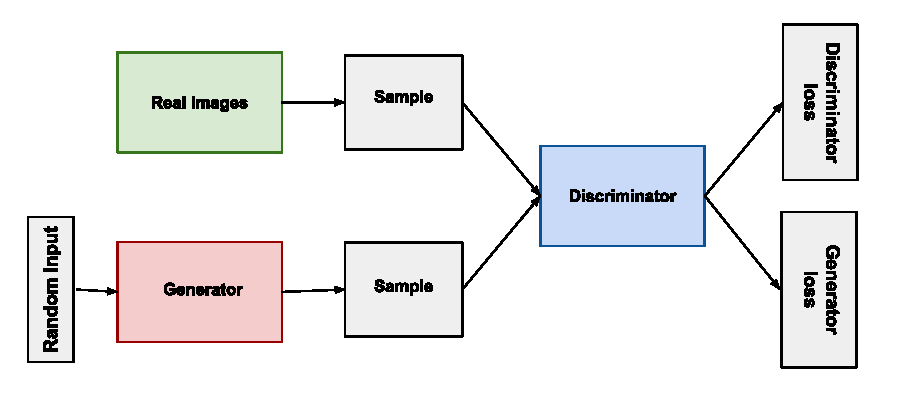
\includegraphics[width=0.75\textwidth]{img/gan/gan_diagram.pdf}
    \caption{Representación gráfica de la arquitectura de una GAN. Imagen obtenida de \cite{googlegan}.}
    \label{fig:gan-diagram}
\end{figure}


\FM[inline]{Si es que en el futuro se puede, modificar esta figura para que coincida más con la descripción}






% El objetivo entonces de la generadora es el de maximizar la función objetivo, mientras que el objetivo de la discriminadora es el de minimizar la función objetivo. En otras palabras, la generadora se entrena para engañar a la discriminadora, y la discriminadora se entrena para clasificar la falsedad de las muestras generadas por la generadora.




% Las Redes Generativas Adversarias (GAN por sus siglas en inglés) son un tipo de arquitectura que se componen de dos partes: un generador $G$ y un discriminador $D$. El objetivo de la generadora $G$ es el de generar muestras que parezcan reales, mientras que el objetivo del discriminador $D$ es el de clasificar las muestras como reales o falsas. En este caso, la red generativa $G$ se entrena para engañar a la red discriminativa $D$, y la red discriminativa $D$ se entrena para detectar las muestras generadas por la red generativa $G$. En la analogía anterior, el ladrón corresponde a la red generativa $G$, y el policía corresponde a la red discriminativa $D$.

% Para lograr este objetivo, la generadora $G$ define una ley $\Prob_G$

% Teorema de la GAN: Convergencia en divergencia Jensen-Shannon

% Ejemplos?
}  % end of sec. Redes Generativas Adversarias


\section{Auto-Encoders}\label{sec:auto-Encoders}
{
    Un tipo de arquitectura que ha sido muy popular por la comunidad del aprendizaje profundo son los Auto-Encoders (AE). Los AE son una arquitectura de redes neuronales que se utilizan para aprender una codificación eficiente de datos no etiquetados. O de forma más coloquial, aprende a ``comprimir la información'' de los datos de entrada.

    Al igual que en la sección anterior, se presentará una definición formal de un AE en el contexto no paramétrico, y utilizando medidas de probabilidad generales. En este caso, esta sección se basa en \cite{tolstikhin2017wasserstein}, aunque ha sido modificado en el contexto de los AE ``vainilla'' (y no en su versión Wasserstein como se presenta en el \textit{paper}).

    Un AE se compone de dos partes: un codificador $Q(\dz \mid x)$ que corresponde a un kernel de transición tal que a cada $x$ le asigna una distribución en el espacio latente, y un decodificador $P_G(\dx \mid z)$ que corresponde a un kernel de transición tal que a cada $z$ le asigna una distribución en el espacio de referencia. En este trabajo, se asume que el decodificador es determinista por simplicidad, es decir, que $P_G(\dx \mid z) = \delta_{G(z)}(\dx)$, donde $G\colon \cZ \to \cX$ es una función.

    Para cumplir con la tarea del aprendizaje de una codificación eficiente, el AE busca minimizar el error de reconstrucción dada una muestra $x\sim \Prob_X$ a través de obtener $\tilde z \sim Q(\dz \mid x)$ y obtener $\tilde x \sim P_G(\dx \mid \tilde z)$. El AE busca minimizar entonces el error de reconstrucción $c(x, \tilde x)$. En este caso, la función de pérdida del AE se define como:
    \begin{equation}\label{eq:ae-loss}
        \cL_{\mathrm{AE}} = \Exp_{X \sim \Prob_X} \Exp_{\tilde Z \sim Q(\dz \mid X)} \left[ c(X, G(\tilde Z)) \right].
    \end{equation}

    En la práctica, uno puede asumir que el codificador es determinista, es decir, que $Q_E(\dz \mid x) = \delta_{E(x)}(\dz)$, donde $E\colon \cX \to \cZ$ es una función que se estima a través de una red neuronal $E_\phi$. Aunque también se puede utilizar un codificador estocástico.
    Por otro lado, el decodificador $P_G(\dx \mid z)$, que se asume determinista en este caso, se estima a través de una red neuronal $G_\theta$.

    De esta manera, el algoritmo para un AE (en su versión más general) se presenta a continuación:
    \begin{algorithm}[tbhp]
        \caption{Auto-Encoder}\label{alg:AE}
        \begin{algorithmic}
            \Require Tamaño del batch $N$.
            \State Inicializar los parámetros del codificador $E_{\phi}$ y del decodificador $G_\theta$.
            \While{$\phi$ y $\theta$ no han convergido}
            \State Muestrear $\{x_i\}_{i=1}^{N} \sim \Prob_X$ desde el conjunto de entrenamiento.
            \State $\tilde z_i \gets E_\phi(x_i)$ para $i=1,\ldots,N$.
            \State $\tilde x_i \gets G_\theta(\tilde z_i)$ para $i=1,\ldots,N$.
            \State Calcular la función de pérdida $\cL_{\mathrm{AE}} = \frac{1}{N}\sum_{i=1}^{N} c(x_i, \tilde x_i)$.
            \State Actualizar $E_\phi$ y $G_\theta$ por medio de descenso de gradiente en $\pdv{\phi} \cL_{\mathrm{AE}}$ y $\pdv{\theta} \cL_{\mathrm{AE}}$.
            \EndWhile
        \end{algorithmic}

    \end{algorithm}




    % En este caso, el AE busca aprender una función $f_{\vth} \colon \cX \to \cX$ tal que $f_{\vth}(x)$ sea parecido a $x$.

    % En este trabajo, se asumirá que el decodificador es determinista, es decir, que $P_G(\dd x \mid z) = \delta_{G(z)}(\dd x)$, donde $G\colon \cZ \to \cX$ es una función que se estima a través de una red neuronal $G_\theta$. Por otro lado, el codificador $Q(\dz \mid x)$ se estima a través de una red neuronal $Q_\phi$.

    % la compresión de datos, la reducción de dimensionalidad, y la generación de datos. En esencia, un AE se compone de dos partes: un codificador $E$ y un decodificador $D$. El objetivo del codificador $E$ es el de mapear una muestra $x$ a un espacio latente $z$, mientras que el objetivo del decodificador $D$ es el de mapear una muestra $z$ de vuelta al espacio original $x$. En otras palabras, el AE busca aprender una función $f_{\vth} \colon \cX \to \cX$ tal que $f_{\vth}(x) \approx x$.

    % Otro tipo de arquitectura que ha sido muy popular en los últimos años son los Auto-Encoders (AE). Los AE son una arquitectura de redes neuronales que se utilizan para la compresión de datos, la reducción de dimensionalidad, y la generación de datos. En esencia, un AE se compone de dos partes: un codificador $E$ y un decodificador $D$. El objetivo del codificador $E$ es el de mapear una muestra $x$ a un espacio latente $z$, mientras que el objetivo del decodificador $D$ es el de mapear una muestra $z$ de vuelta al espacio original $x$. En otras palabras, el AE busca aprender una función $f_{\vth} \colon \cX \to \cX$ tal que $f_{\vth}(x) \approx x$.
}  % end of sec. Auto-Encoders


}  % end of Chapter Modelos Generativos